% Template ripped from:
% http://www.cs.technion.ac.il/~yogi/Courses/CS-Scientific-Writing/examples/simple/simple.htm

\title{Differential Privacy with Dependent Types}
\author{
        Casper Holmgreen \\
        Department of Computer Science\\
        DIKU - Datalogisk Institut, K\o benhavns Universitet\\
        \and
        Knut Liest\o l\\
        Department of Computer Science\\
        DIKU - Datalogisk Institut, K\o benhavns Universitet\\
}
\date{\today}

\documentclass[12pt]{article}

\usepackage{graphicx}
\usepackage{listings}
\usepackage{amsfonts,amsthm,amsmath}

\newtheorem{defn}{Definition}[section]

\begin{document}
\maketitle

\lstset{language=Haskell,basicstyle=\footnotesize,frame=single,
        numbers=left}

\begin{abstract}
This is the paper's abstract \ldots
\end{abstract}

\section{Introduction}\label{sec:introduction}

With each passing day, more and more of our personal information is being collected, cataloged and analyzed by an ever increasing number of interested parties.
Their interests can range from targeted advertising to malicious and potentially illegal actions and everything in between.
As the producers of this data, we should be concerned with how it is being used.

[maybe copy paste the rest of this from the original?]

\section{Dependent Types in Idris}\label{sec:dependent_types_in_idris}

Concepts used later in the paper that need to be defined here:
\begin{itemize}
\item Idris data constructors cannot share names with type constructors
\item Very small segment about sections (e.g. \texttt{(*10)})
\item TBD
\end{itemize}

\section{Differential Privacy}\label{sec:differential_privacy}

In this section, we describe the central ideas and metrics behind differential privacy.

\section{Function Sensitivity}\label{sec:function_sensitivity}

Function sensitivity plays a central role in much of the differential privacy literature.
We can make assertions about an entire program if we understand the sensitivities of the functions with which it is composed.
In this section, we describe function sensitivity and then demonstrate how we use dependent types to model it in Idris.

Function sensitivity captures the idea of how relatively ``far'' a function can magnify the distance between pairs of inputs.
We say that a function is $c$-sensitive if, for all pairs of inputs, the distance between the outputs is not $c$ times greater than the original distance between the inputs.

	$$ \forall x,y. d(f(x),f(y)) \le c \times d(x,y) $$

For example, imagine a function $f : \mathbb R \rightarrow \mathbb R$ and Euclidian distance function $d_{\mathbb R}(x,y) = |x-y|$.
Now sample two random values from a 1D line: $x,y$.

Consider the case where $f(x) = \texttt{add10}(x) = x + 10$.
Clearly, it doesn't matter which $x$ and $y$ you sample; the distance $d_{\mathbb R}(x,y)$ will always equal $d_{\mathbb R}(f(x),f(y))$.
We say that \texttt{add10} is a 1-sensitive function.
Now consider the case where $f(x) = \texttt{doubleThenAdd10}(x) = 2x + 10$.
Distances can be now be doubled (but no more), so it is a 2-sensitive function.
Intuitively, when dealing with linear functions and the Euclidian distance function, the largest linear coefficient will dictate the c-sensitivity.
Higher order polynomials can be only be described as being $\infty$-sensitive.

Linear functions and Euclidian distances are not terribly interesting.
Function sensitivity applies to many other interesting domains such as databases containing private tax records or health information.

We will use $\mathbb D$ to describe the domain of databases.
Hence, a function $f : \mathbb D \rightarrow \mathbb D$ is a function across databases.
Our distance function will just be the symmetric difference of two databases; i.e. $d_{\mathbb D}(D_1,D_2) = | D_1 \oplus D_2 |$.
There is a common case in the differential privacy literature where two databases differ by exactly 1 row (i.e. $d_{\mathbb D}(D_1,D_2)=1$).
This is notationally represented by $D_1 \sim D_2$.

Function sensitivies compose, too.
The composition of \texttt{add10 . doubleThenAdd10} is 2-sensitive.
\texttt{doubleThenAdd10 . doubleThenAdd10} is 4-sensitive.
Function sensitivity represents the maximum multiplicative factor by which the distances can increase.
So it follows that the composition of two functions, $f$ and $g$, which are $c$- and $c'$-sensitive, respectively, will be $(c \times c')$-sensitive.

% TODO : discuss any function that is c-sensitive is also c'-sensitive, for all $c < c'$.

\subsection{Function sensitivity in Idris}

Modelling function sensitivity in Idris is simple.
Obviously we will need to index the type by sensitivity.
To keep this example simple, we will use \texttt{Float} to represent it, but our implementation uses an implementation of \texttt{Rational}s, which should be numerically more stable than IEEE floating point numbers.

We define a type constructor indexed by the sensitivity, input and output types, with just one data constructor for wrapping native functions.

\begin{lstlisting}
data SensitiveFunction : Float -> Type -> Type -> Type where
    MkSensitiveFunction : (a -> b) -> SensitiveFunction s a b

namespace Examples

    add10 : SensitiveFunction 1 Float Float
    add10 = MkSensitiveFunction (+10)

    doubleThenAdd10 : SensitiveFunction 2 Float Float
    doubleThenAdd10 = MkSensitiveFunction (*2)

    cheat : SensitiveFunction 1 Float Float
    cheat = MkSensitiveFunction (*20)
\end{lstlisting}

Notice the \texttt{cheat} example above.
It is possible to define so-called ``sensitive functions'' which intentionally misrepresent themselves.
Our focus here is not on the verification of a function's sensitivity, but rather on the interaction between sensitivity and the type system under operations such as function composition or application.
Unrestricted application is as simple as unwrapping the function and applying it.
Composition returns a new data constructor indexed on the appropriate sensitivity.

\begin{lstlisting}
apply : SensitiveFunction s a b -> a -> b
apply (MkSensitiveFunction f) x = f x

(.) : SensitiveFunction s b c -> SensitiveFunction s' a b -> SensitiveFunction (s*s') a c
(.) (MkSensitiveFunction g) (MkSensitiveFunction f) = MkSensitiveFunction (g . f)
\end{lstlisting}
% TODO: Fix text running off page

\section{Typing the Relational Algebra}\label{sec:typing_the_relational_algebra}

In this section, we review the relational algebra and show how it can be modelled in a dependently typed language.
Our approach is based on \cite{OurySwierstra08PowerOfPi}.

The relational algebra describes semantics for modelling and querying data in relational databases (e.g. MySQL\footnote{https://www.mysql.com/}).
E.F. Codd described relational databases and their associated algebra back in the 1970's.
% TODO : find reference to paper
The relational model quickly became popular for its simplicity and good performance.

In the relational algebra, relations are modelled as tables.
The rows of a table represent individual entities and the columns represent their attributes.
Each of these columns is associated with a data type.
Every table has a \textit{schema}, which is the last of its column names and types.
For example, the table below contains four columns; each has a unique name and an associated data type.

\begin{table}[tb]
    \caption{caption here}
    \label{tab:tablename}
    \centering

    \begin{tabular}{|c|c|c|c|}
    \hline

    \hline
    \textbf{Key} & \textbf{Name} & \textbf{Age} & \textbf{FavoriteFood} \\
    \hline
    \textit{Int} & \textit{String} & \textit{Int} & \textit{String} \\
    \hline
    \hline
       1 & Casper & 26 & Chicken Curry \\
       2 & Knut & 26 & ??? \\
       % TODO : Knut fills out fav. food
    \hline

    \end{tabular}
\end{table}

The relational algebra allows us to build structured queries against relational databases.
The primary operators are listed below.
Note that some of the operators may require expressions to be provided (e.g. for filtering a table with a conditional).

\begin{itemize}
    \item selection
    \item projection
    \item Cartesian product\footnote{\label{fn:set_ops} These operations function identically to their set counterparts, but impose additional requirements regarding table schemas. In particular, union and difference (and therefore intersection) require that the schemas of the two operands match. The Cartesian product operator requires that the two schemas are disjoint.}
    \item set union\footnotemark[\ref{fn:set_ops}]
    \item set difference\footnotemark[\ref{fn:set_ops}]
\end{itemize}

Note that the set operations and Cartesian product impose additional requirements in this context.
They have precluded many type systems from being able to fully type-check the relational algebra.
Strongly-typed languages, such as Haskell, have devised clever solutions to this problem, but none are as straight-forward as the approach available to a dependent type system.
The ability to capture schemas directly in the types and to manipulate them yields a deceptively simple, but powerful typing framework for relational databases.

\subsection{Relational Algebra in Idris}

This section will briefly outline a simple implementation of the relational algebra in Idris.
We begin by defining some simple algebraic datatypes (ADTs) for keeping the types clear.
We then define a toy expression language before defining the query language.

First, we need to be able to represent table attributes (columns).
An attribute is just the pairing of a name and a data type.
Following David Christiansen's lead, we opt to use \texttt{(:::)} instead of the more traditional \texttt{(,)} for constructing our pairs.
We believe this enhances readability of long schemas, which are just lists of attributes.

\begin{lstlisting}
data Attribute : Type where
  (:::) : String -> Type -> Attribute

Schema : Type
Schema = List Attribute

namespace Examples

    people : Schema
    people = [ "Key"          ::: Int 
             , "Name"         ::: String
             , "Age"          ::: Int
             , "FavoriteFood" ::: String
             ]
\end{lstlisting}

The relational algebra assumes the existence of an expression language, so we implement a primitive one for demonstration.
An expression will have access to all of the attributes of a row during evaluation and will return a value of some arbitrary type.
Thus, an expression with the type \texttt{Expr s a} can be read as an expression with access to the attributes in schema \texttt{s} returning type \texttt{a}.
Notice that we have not yet defined any underlying representation for the rows.
% TODO : expand on this idea

\begin{figure}[tb]
    \centering
    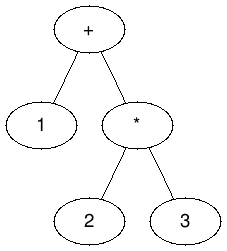
\includegraphics[]{assets/expr_tree.png}
    \caption{Caption here}
    \label{fig:figure1}
\end{figure}
% TODO : resize and work with this graph. write about it in the neighboring text

Expressions can be built up from other expressions, forming an expression tree.
What type will a complex expression tree have?
Expressions cannot change the schema, so it must remain constant even as we grow the tree.
The root of the tree represents the last ``operation'' to be applied under evaluation.
The return type of the root of the tree is the return type of the tree.
Only well-typed expression trees will be allowed by the type checker.

\begin{lstlisting}
data Expr : Schema -> Type -> Type where
    (^)    : (s:Schema) -> (nm:String) -> { auto p : (map cast s) `ContainsKey` nm } -> Expr s (lookupType s p)
    (+)    : Num t => Expr s t -> Expr s t -> Expr s t
    (==)   : Eq t  => Expr s t -> Expr s t -> Expr s Bool
    Lit    : t -> Expr s t
    PureFn : (a -> b) -> Expr s a -> Expr s b

namespace Examples

    fountain_of_youth : Expr s Int
    fountain_of_youth = people^"Age" - 10
\end{lstlisting}

The \texttt{PureFn} data constructor lifts pure Idris functions into the expression language, which should allow programmers to bend even this toy expression language to the task at hand.
Unfortunately, this functionality is only available to the Idris backend.
% TODO: true?
\texttt{ContainsKey} is just a proof that the given schema contains the attribute in question.
It is derived automatically, so users of our language should never have to worry about it.
\texttt{lookupType} is able to use this proof to statically verify the types.

% TODO : insert image of expr AST

The core of the relational algebra consists of the query operators.
They are modelled as follows.
Note that \texttt{Query} is a data family.
This allows us to adjust its data representation just enough to implement a variety of backends.
The leaves of all queries will be very backend specific.
An in-memory Idris backend might store pointers to the tables directly in the data constructor, whereas a SQL backend might just store the name of the table.
One of the benefits of this is that any dataset which can be modelled using the relational algebra is usable.

\begin{lstlisting}
mutual
    data Query : (Schema -> Type) -> Schema -> Type where
        Table   :       t s -> Query t s
        Union   : Query t s -> Query t s -> Query t s
        Diff    : Query t s -> Query t s -> Query t s
        Product : Query t s -> Query t s' -> { auto p : Disjoint s s' } -> Query t (s ++ s')
        Projection : (f:String -> Maybe String) -> Query t s -> Query t (projectedSchema f s)
        Select  : Expr s Bool -> Query t s -> Query t s
    data Grouping : (Schema -> Type) -> Schema -> Type -> Type where
        GroupBy : Eq k => Expr s k -> Query t s -> Grouping t s k
    data Partitioning : (Schema -> Type) -> Schema -> Type -> Type where
        Partition : Eq k => List k -> Expr s k -> Query t s -> Partitioning t s k
\end{lstlisting}

Recall that the set operators require additional constraints that less powerful type systems have a difficult time capturing.
Set union and difference require that the two operands share matching schemas.
Cartesian product requires that they be disjoint.
We just use type unification to express the first two and a machine-decidable proof of disjointness for the other.

% TODO : write about backends

\section{Our implementation}\label{sec:our_implementation}

In this section, we describe how we bring together the material of the previous chapters and outline our entire implementation.

Our goal is to leverage Idris's type-checker to statically verify differential privacy constraints.
We create new types to capture the necessities.
We will focus on \texttt{PINQuery} because the other two have similar implementations, but are case-specific.

\begin{lstlisting}
data PINQuery : (Schema -> Type) -> Schema -> Stability -> Type where
    MkPINQuery : Query t s -> PINQuery t s c
data PINGrouping : (Schema -> Type) -> Schema -> Type -> Stability -> Type where
    MkPINGrouping : Grouping t s k -> PINGrouping t s k c
data PINPartitioning : (Schema -> Type) -> Schema -> Type -> Stability -> Type where
    MkPINPartitioning : Partitioning t s k -> PINPartitioning t s k c
\end{lstlisting}

% TODO 1 : discuss transformation stability vs. function sensitivity

A \texttt{PINQuery t s c} describes a \texttt{c}-differentially private query with schema \texttt{s} (and backend table representation \texttt{(t s)}).
There is only one data constructor which serves simply to wrap a \texttt{Query}, which was defined in Section~\ref{sec:typing_the_relational_algebra}.
This allows us to define a \texttt{Query} and assign it an arbitrary stability.

Next, we provide the standard operators from the relational algebra.
This time, however, we do not build up abstract syntax trees with ADTs.
That approach proved to be unnecessarily complex with regards to satisfying the type-checker.
% TODO 2 : probably expand on this point
Instead, we unwrap the \texttt{Query} and then rewrap it in the same data constructor, but using a different type constructor.
This is because the schema and stability could potentially change.
We control the API that is exported, so we carefully implement the relational algebra operators with the correct stability costs.
% TODO 3 : make the PINQuery ADT abstract
By unwrapping and rewrapping the \texttt{Query} trees from Section~\ref{sec:typing_the_relational_algebra} in our new type, we are now able to build query trees that carry privacy metrics in the type.

\begin{lstlisting}
where' : PINQuery b s c -> Expr s Bool -> PINQuery b s c
where' (MkPINQuery q) e = MkPINQuery (Select e q)

select : PINQuery b s c -> (f:String -> Maybe  String) -> PINQuery b (projectedSchema f s) c
select (MkPINQuery q) f = MkPINQuery (Projection f q)

union : PINQuery b s c -> PINQuery b s c' -> PINQuery b s (c + c')
union (MkPINQuery q) (MkPINQuery q') = MkPINQuery (Union q q')

intersect : PINQuery b s c -> PINQuery b s c' -> PINQuery b s (c + c')
intersect (MkPINQuery q) (MkPINQuery q') = MkPINQuery (Diff q q')

groupBy : Eq k => Expr s k -> PINQuery b s c -> PINGrouping b s k (c * 2)
groupBy e (MkPINQuery q) = MkPINGrouping (GroupBy e q)
\end{lstlisting}

\texttt{where'} is a 1-sensitive function and it's type declaration reflects that.
% TODO 2 : give proof
The \texttt{c} parameter remains unchanged through the rewrapping.

\texttt{union}, however, costs the sum of the costs of the operands.
Notice how easily this is described in Idris.

Of course, we can't just return the results of any query.
A query might just return the database contents untouched, potentially violating every single participant's privacy.
Differential privacy essentially requires that any query response be the result of some sort of aggregation.

Additionally, the control flow of a program may be predicated on the value returned from an aggregation.
Sequential queries are additive in cost.
Sequencing computations in functional programming is traditionally accomplished using the infamous \texttt{Monad}.
In many languages, Idris included, types implementing \texttt{Monad} instances have access to special syntactic sugar, commonly known as \texttt{do}-notation.
It is important to note that \texttt{do}-notation is not magic!
It just allows developers an alternative method for writing monadic code.

We want to take advantage of this, but the type signatures required to satisfy a monad instance preclude our ability to reflect sensitivities in the types.
Fortunately, Idris does not actually require a \texttt{Monad} instance to overload \texttt{do}-notation.
We just need to provide the functions \texttt{(>>=)} and \texttt{return}.

\begin{lstlisting}
data Private : Sensitivity -> Type -> Type
    MkPrivate : (CrapGen -> (a,CrapGen)) -> Private budget a

return : a -> Private 0 a
return x = MkPrivate $ \s => (x,s)

(>>=) : Private s a -> (a -> Private s' b) -> Private (s + s') b
(>>=) (MkPrivate sf) f = MkPrivate $ \st => let (x,st1)       = sf st
                                                MkPrivate sf' = f x
                                             in sf' st1

evalPrivate : Private s a -> CrapGen -> a
evalPrivate (MkPrivate f) g = fst (f g)

namespace Examples

    nestedAggregations : Private 3 Double
    nestedAggregations = do x <- the (Private 1 Double) someAggregation
                            y <- the (Private 2 Double) someOtherAggr
                            return ((x+y*2)/3)
\end{lstlisting}

Experienced functional programmers will probably recognize that \texttt{Private} is functionally equivalent to a \texttt{State} monad instance.
Laplace noise requires pseudorandom number generation, so we are keeping track of a generator throughout the computation.

Each aggregation is responsible for providing differential privacy.
Our implementation provides several common aggregations, such as \texttt{noisyCount} and \texttt{noisyAverage}.
Experts will be able to write their own aggregations to provide to the public.

Of course, aggregation alone is not sufficient for guaranteeing privacy.
We must add Laplace noise according to the sensitivity of the \texttt{PINQuery} and a user-provided epsilon.

\texttt{noisyCount} is a good example of a simple aggregation.
The user provides a \texttt{PINQuery} (which has an associated stability cost) and an arbitrary epsilon reflecting how accurate they want the result to be.
The added noise is scaled according to the user provided epsilon while the privacy cost of the entire computation is computed in the types.

\begin{lstlisting}
noisyCount : (PINQuery Table s c) -> (e:Epsilon) -> Private (c*e) Double
noisyCount (MkPINQuery q) eps = MkPrivate $ \g => 
  let (rx,g') = rndDouble g
      noise   = samplePure 0 (1 / toFloat eps) rx
      count   = the Double $ fromInteger $ fromNat $ length (eval q)
   in (count + noise, g')
\end{lstlisting}

\section{Evaluation}\label{sec:evaluation}

In this section we will present our results. More specifically, we will compare DPINQ to our inspirational library, PINQ.

\subsection{API and flexibility}

In order for a query language to be useful, it should be flexible, such that it can be used to express a range of algorithms. Differential privacy guarantees limits the flexibility in comparison to query languages without privacy concerns. Therefore, we have concidered flexibility to be an important success criteria for us.

PINQ is fairly flexible considering its privacy guarantees. It is achieved by implementing simple primitives that are guaranteed to be differentially private, which can be mixed and matched together.
PINQ also gets a lot of flexibility from the fact that it is built on top of LINQ, which grants users access to the powerful expression language of LINQ. This has its downside when it comes to safety though, which will be discussed later.

Our language has the same API as PINQ, but currently lack some of the flexibility PINQ provides. For our Idris backend, the expression operation \texttt{PureFn} provides flexible expressions only limited by Idris' capabilities, as it lifts an arbitrary Idris function to our expression language. 
Unfortunately we are unable to compile an arbitrary Idris function to SQLite, so this functionality is not supported by our SQLite backend. This means that there are algorithms that can be written in our language using the Idris backend, but not using the SQLite backend. 
We describe a possible solution in Future work to grant more flexibility to external database backends. 

Some algorithms are also inherently more difficult to represent in a dependently typed language than in languages with more limited type systems. An example is a k-means algorithm with a dynamic termination. The standard k-means algorithms runs for \texttt{n} iterations. Another version is one where the algorithm terminates based on some condition, e.g. that half of the remaining budget is used every iteration until some defined convergence point. This algorithm is difficult to represent in a dependent type system.

\subsection{Type safety and security}

For all practical purposes, LINQ is type safe. It has powerful lambda expressions that use the data source schema to reference fields with type safety. 
PINQ only validates privacy constraints dynamically, which means that users can write valid PINQ programs that violate privacy constraints.

With Idris' flexible type system, we were able to make our language completely type safe, as described in the Power of Pi section.
As we perform privacy calculations on the type level, users of our language are unable to write valid programs that violates privacy constraints.

As mentioned in the previous subsection, PINQ allows users access to powerful LINQ lambda expressions. This freedom comes at the cost of security. Because the expressions has the whole .NET runtime at its disposal, side-channel attacks are possible. An example could be an expression that sends the raw, sensitive data off to a remote database. A rewrite function intended to remove such unsafe code from expressions is planned, but not implemented in the current version of PINQ.

Side-channel attacks is not a problem in our language due to the pure nature of Idris. It is simply impossible to create side-effecting functions without specifically defining an effectful function, which can not be called by another function unless also that function is effectful.

\section{Discussion}\label{sec:discussion}

In this section, we evaluate our language and discuss various things about it.

\section{Conclusion}\label{sec:conclusion}

We worked very hard, but achieved very little.

\bibliographystyle{abbrv}
\bibliography{main}

\end{document}
